\documentclass[9pt]{IEEEtran}

\usepackage[english]{babel}
\usepackage{graphicx}
\usepackage{epstopdf}
\usepackage{fancyhdr}
\usepackage{amsmath}
\usepackage{amsthm}
\usepackage{amssymb}
\usepackage{url}
\usepackage{array}
\usepackage{textcomp}
\usepackage{listings}
\usepackage{hyperref}
\usepackage{xcolor}
\usepackage{colortbl}
\usepackage{float}
\usepackage{gensymb}
\usepackage{longtable}
\usepackage{supertabular}
\usepackage{multicol}

\usepackage[utf8x]{inputenc}

\usepackage[T1]{fontenc}
\usepackage{lmodern}{}
\input{glyphtounicode}
\pdfgentounicode=1

\graphicspath{{./figures/}}
\DeclareGraphicsExtensions{.pdf,.png,.jpg,.eps}

% correct bad hyphenation here
\hyphenation{op-tical net-works semi-conduc-tor trig-gs}

% ============================================================================================

\title{\vspace{0ex}
Correlation filter tracking}

\author{Marko Medved\vspace{-4.0ex}}

% ============================================================================================

\begin{document}

\maketitle

\section{Introduction}
In this assignment, we implemented the Correlation Filter tracker and tested its performance on the VOT 
2014 dataset using the Tracking Toolkit-lite. We then utilized the Toolkit to determine the optimal parameters
 for the tracker. Following this, we evaluated the tracking speed across different sequences and compared the
  average initialization time with the average tracking time. All measurements were performed on an AMD Ryzen 
  7 7435HS CPU. Finally, we enhanced the tracker by implementing the MOSSE tracker, which updates the numerator
   and denominator of the correlation filter separately for improved performance, and also affects the updates
   with the PSE measure.

\section{Experiments}
\subsection{Base tracker performance results}
The simplified correlation filter tracker was first implemented and evaluated using the Tracking Toolkit-lite 
and the VOT 2014 dataset. The results can be seen in Table~\ref{tab:corr_tracker_results}. For this evaluation, 
the following parameters were used: $\sigma=1.5$, which corresponds to the Gaussian parameter, and $\alpha = 0.3$, 
representing the update speed. Additionally, the regularization parameter was set to 2000, a value consistent across 
all evaluations in this assignment.


\begin{table}[ht]
  \centering
  \caption{Performance of the basic correlation filter tracker.}
  \begin{tabular}{l|c}
  \hline
  \textbf{Metric}            & \textbf{Value}        \\
  \hline
  Average Overlap            & 0.51                  \\
  Total Failures             & 61.0                    \\
  Average Speed (FPS)        & 1052.08            \\
  \hline
  \end{tabular}
  \label{tab:corr_tracker_results}
  \end{table}

  \subsection{Testing different parameters}
  To enhance the tracker's performance, various values for $\sigma$ and $\alpha$ were tested.

  Figure~\ref{fig:alpha} shows how the total failures and average overlap vary with different values 
  of $\alpha$. The results indicate that $\alpha = 0.15$ produced the lowest number of failures, with 56,
   while $\alpha = 0.05$ was a close second with 58 failures. Importantly, $\alpha = 0.05$ also achieved a
    higher average overlap, making it the optimal choice for the parameter. This suggests that updating the
     template at a slower rate is beneficial, though not as slowly as with the previously implemented mean-shift tracker.

  \begin{figure}[h]
    \centering
    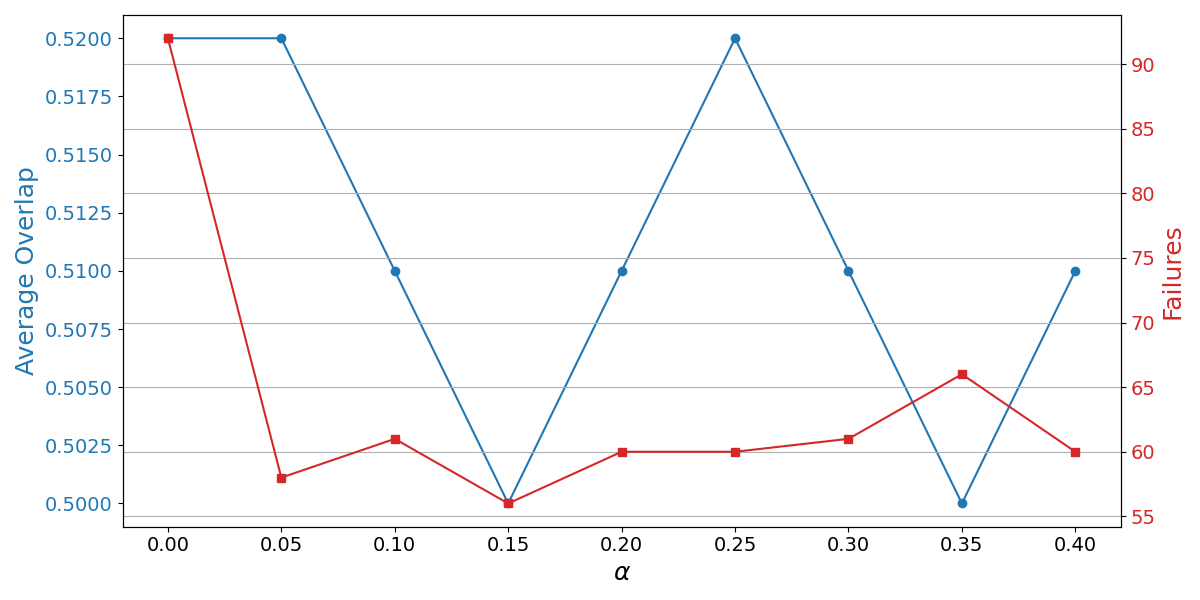
\includegraphics[width=0.99\columnwidth]{figures/tracking_alpha.png}
    \caption{Comparison of the tracker with different update speeds}
    \label{fig:alpha}
\end{figure}

Secondly, Figure~\ref{fig:sigma} shows that the tracker's performance is also sensitive to changes in
 $\sigma$. The lowest number of failures occurs at $\sigma = 2.25$, with 57 failures. However, $\sigma = 1.5$
  is only slightly worse with 58 failures, and it also provides the best average overlap. Therefore, $\sigma = 1.5$
   is considered the optimal value for this parameter. 

   \begin{figure}[h]
    \centering
    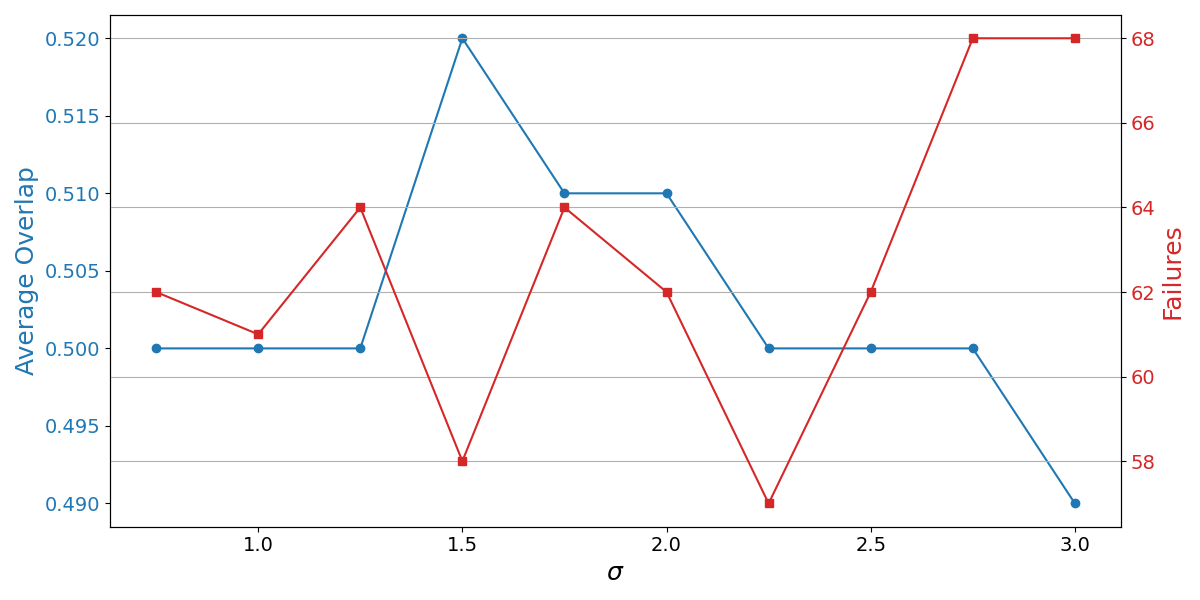
\includegraphics[width=0.99\columnwidth]{figures/tracking_sigma.png}
    \caption{Comparison of the tracker performance with different standard deviations 
    of the Gaussian}
    \label{fig:sigma}
  \end{figure}

  \subsection{Testing larger patches}
  For the next experiment, we explored the use of a larger template. The performance of the tracker across
   different enlargement factors is shown in Figure~\ref{fig:enlargement}. From the plot, it is clear that the
    average overlap decreases as the enlargement factor increases. Interestingly, the number of failures decreases
     at certain factors (1.05 and 1.2). The decrease in overlap could be attributed to the tracker template updating 
     with each frame, causing the tracker to focus not only on the target but also on surrounding background elements,
      which reduces the overlap. On the other hand, the reduction in failures at certain enlargement factors suggests
       that tracking the background can be beneficial when the background moves in tandem with the target. It 
       is important to note that a larger background generally results in slower tracker performance. 
       Note that for further evaluation the enlargement factor of 1.20 will be used, since it 
       produces the smallest amount of failures on the dataset, while also retaining a pretty good 
       average overlap. 

  \begin{figure}[h]
    \centering
    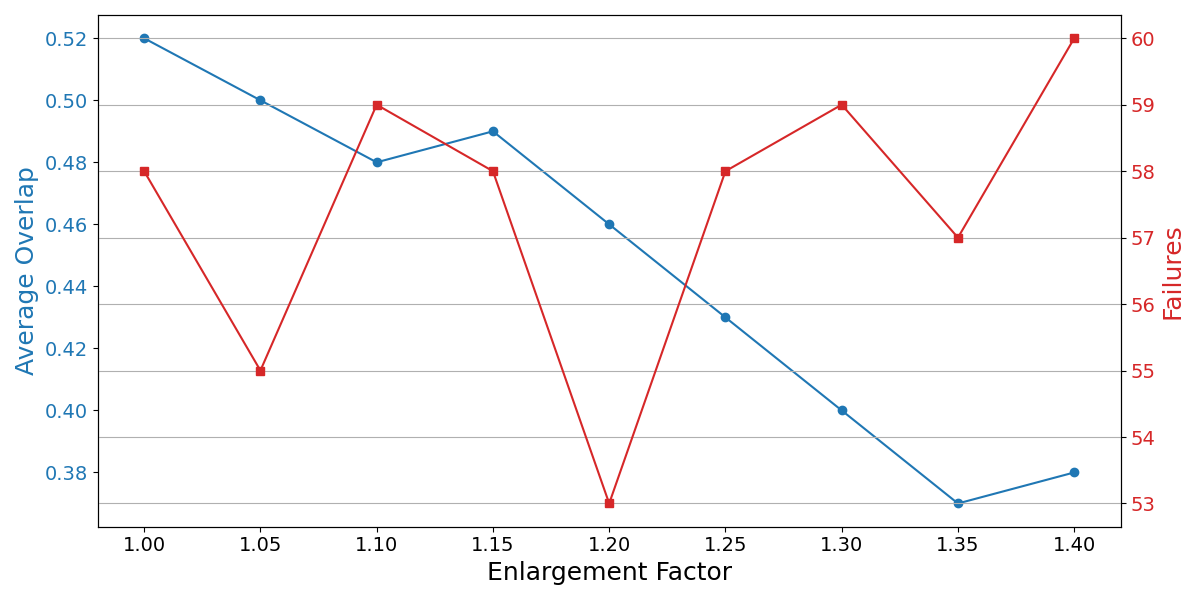
\includegraphics[width=0.99\columnwidth]{figures/tracking_enlargement.png}
    \caption{Comparison of the tracker performance with different background 
    enlargement factors}
    \label{fig:enlargement}
  \end{figure}

\subsection{Tracking speed evaluation}
We evaluated the tracking speed performance across all sequences from the VOT 2014 dataset, as shown
 in Figure~\ref{fig:tracking_speed}. A notable variation in tracking speeds can be observed across the sequences, 
 which can be attributed to several factors. The most apparent factor is the size of the patches in each sequence.
  For instance, the sequence "surfing," which has a small patch, exhibits the fastest tracking speed, while "motocross,"
   with a larger patch, has the slowest tracking speed.

Another contributing factor is the number of tracker failures. To better understand the impact of these failures,
 we calculated the average initialization speed and the average track speed for the entire dataset, which were found 
 to be 1119.97 FPS and 808.46 FPS, respectively. Interestingly, this suggests that the number of failures may actually
  speed up the tracker. In light of this, a more accurate comparison would focus solely on track speeds, excluding the
   initialization frames. This comparison is presented in Figure~\ref{fig:tracking_speed2}, where, although the changes in 
   the order of sequences are minor, they are still noticeable.

\begin{figure}[h]
  \centering
  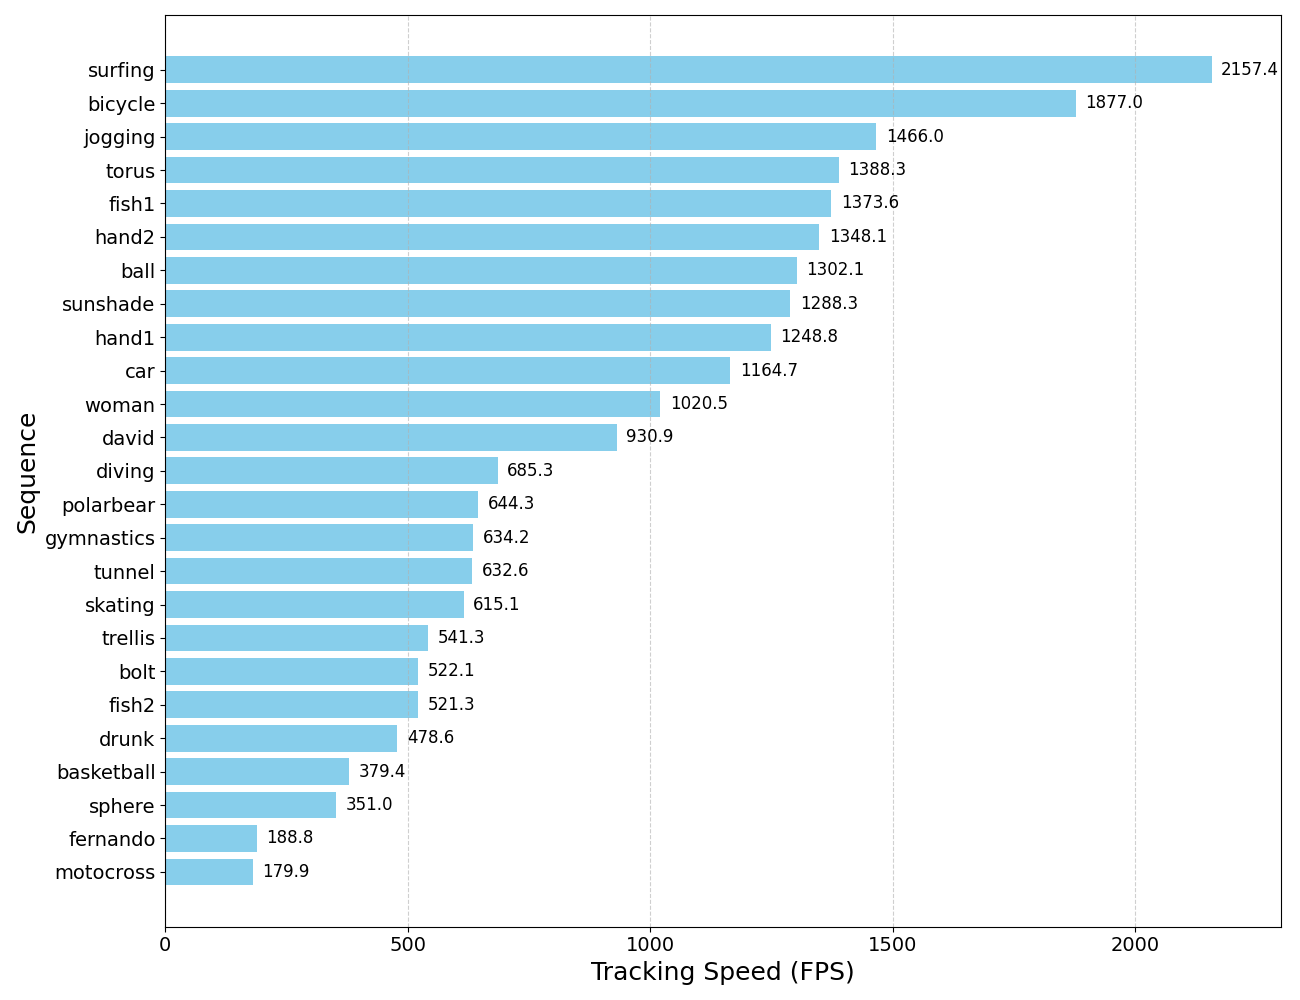
\includegraphics[width=0.99\columnwidth]{figures/tracking_speed.png}
  \caption{Comparison of the tracking speed (initialization frames included) across sequences in the VOT 2014 dataset}
  \label{fig:tracking_speed}
\end{figure}


\begin{figure}[h]
  \centering
  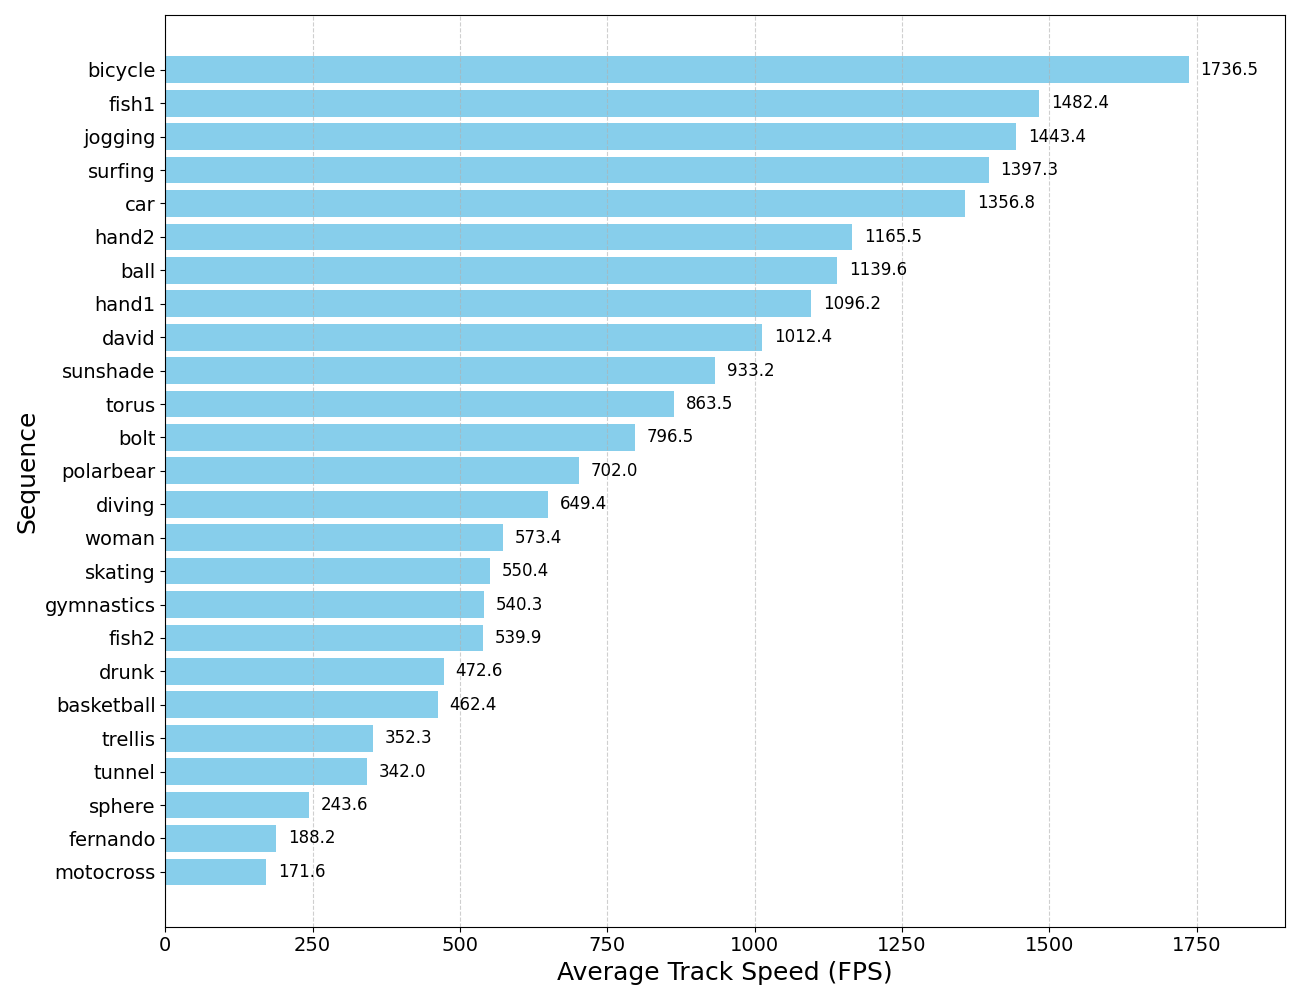
\includegraphics[width=0.99\columnwidth]{figures/average_track_speed.png}
  \caption{Comparison of the tracking speed (no initialization frames included) across sequences in the VOT 2014 dataset}
  \label{fig:tracking_speed2}
\end{figure}

\subsection{MOSSE tracker}
We implemented the actual MOSSE tracker, which updates the numerator and denominator of 
the correlation filter separately. Additionally, we integrated the PSR (Peak Signal-to-Noise Ratio)
 measure for occlusion detection and tested various PSR thresholds to determine when the filter
  should update. The optimal threshold was found to be 4.0. For the PSR calculation, we used a window
   size of 11, which defines the area around the maximum value that should be excluded from the
    calculation.

As shown in Table~\ref{tab:mosse_tracker_results}, the number of failures decreased slightly
 (from 53 to 51), while the average overlap remained unchanged. It is also important to note 
 that the average speed of the tracker decreased as expected, due to the additional operations 
 introduced by the PSR measure. 

\begin{table}[h!]
  \centering
  \caption{Tracker performance for \texttt{mosse\_tracker}}
  \begin{tabular}{l|l}
  \hline
  \textbf{Metric}            & \textbf{Value} \\ \hline
  Average overlap            & 0.46           \\ \hline
  Total failures             & 51.0           \\ \hline
  Average speed (FPS)        & 686.92         \\ \hline
  \end{tabular}
  \label{tab:mosse_tracker_results}
  \end{table}
  

\section{Conclusion}
In this assignment, we implemented and tested the correlation filter tracker, demonstrating that 
optimizing the tracker parameters significantly affects its performance. We also showed that using a
 larger template could be beneficial in certain cases. Additionally, we observed that tracking speed 
 can vary greatly based on the size of the patches and the number of tracker failures.

Lastly, we implemented the MOSSE tracker, which further improved the performance by updating the correlation
 filter’s numerator and denominator separately, and by integrating the PSR measure for occlusion detection.
  Despite these improvements, the MOSSE tracker did not outperform the previously implemented mean-shift tracker.

To further improve the tracker multiple enhancements are possible, including scale adaptation and leveraging multichannel 
tracking to handle more complex scenarios effectively.



\bibliographystyle{IEEEtran}
\bibliography{bibliography}

\end{document}
